\documentclass[11pt,a4paper]{article}
\usepackage[T1]{fontenc}
\usepackage{isabelle,isabellesym}
\usepackage{amssymb}
\usepackage{tikz}
\usepackage{float}
\usepackage[most]{tcolorbox}
\usepackage{pdfsetup}

\urlstyle{rm}
\isabellestyle{it}

% One coloured box per kind of declaration (the theory wraps each declaration in one of them).
\newcommand{\declbox}[4]{%
  \newtcolorbox{#1}[1]{enhanced, breakable, colback=#2!4, colframe=#2!60!black, boxrule=0.6pt,
    arc=2mm, left=2mm, right=2mm, top=1mm, bottom=1mm, before skip=2mm, after skip=2mm,
    fonttitle=\sffamily\bfseries\footnotesize, coltitle=white, colbacktitle=#2!60!black,
    title={#3\ \texttt{##1}}, #4}}
\declbox{defbox}{blue}{Definition}{}
\declbox{lembox}{green!50!black}{Lemma}{}
\declbox{thmbox}{orange}{Theorem}{}
\declbox{databox}{gray}{Data / certificate}{}
\declbox{ctrlbox}{violet}{Negative control}{}

\begin{document}

\title{Integer Frieze Patterns with Strictly Ordered Middle Rows}
\author{Carles Mar\'in}
\maketitle

\begin{abstract}
Tabachnikov asked whether, for two frieze patterns of positive numbers of the same width, the differences
of the entries of a fixed row must change sign at least four times along the period. Cuntz found a
counterexample with rational entries, and the case of frieze patterns of positive integers
(Conway--Coxeter friezes) was left open. We formalize an infinite family of integer counterexamples: for
every even $n \geq 14$, two Conway--Coxeter frieze patterns of width $n - 3$ whose middle rows are strictly
ordered at every position, so that their difference has no sign change at all. Frieze patterns are
represented by unimodular lattice polygons. We prove that inserting an ear preserves them, that their
entries are continuants of the quiddity, and that inserting ears at two antipodal positions preserves the
strict order of the middle rows when a polynomial inequality holds, as it does along the family.
\end{abstract}

\paragraph{Acknowledgement.} The formalization and the text of this document were prepared with the
assistance of the AI system Claude (Opus 5.5, Anthropic), and checked by the author. The computer search
that found the pair for $n = 14$, and the exhaustive check that no smaller width has two integer frieze
patterns with strictly ordered rows, were done outside Isabelle and are not part of this entry.

% generated by research/frisos-sturm/figura_afp.py (Curiosity); do not edit by hand
\begin{figure}[H]
\centering
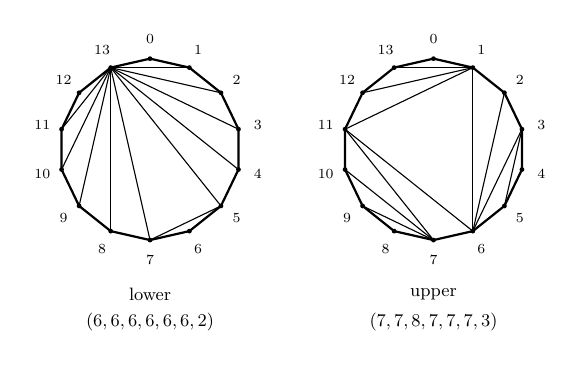
\begin{tikzpicture}[scale=0.72, every node/.style={transform shape}]
  % lower
  \draw[thick] (0.000,1.600) -- (0.694,1.442) -- (1.251,0.998) -- (1.560,0.356) -- (1.560,-0.356) -- (1.251,-0.998) -- (0.694,-1.442) -- (0.000,-1.600) -- (-0.694,-1.442) -- (-1.251,-0.998) -- (-1.560,-0.356) -- (-1.560,0.356) -- (-1.251,0.998) -- (-0.694,1.442) -- cycle;
  \draw (0.694,1.442) -- (-0.694,1.442);
  \draw (1.251,0.998) -- (-0.694,1.442);
  \draw (1.560,0.356) -- (-0.694,1.442);
  \draw (1.560,-0.356) -- (-0.694,1.442);
  \draw (1.251,-0.998) -- (0.000,-1.600);
  \draw (1.251,-0.998) -- (-0.694,1.442);
  \draw (0.000,-1.600) -- (-0.694,1.442);
  \draw (-0.694,-1.442) -- (-0.694,1.442);
  \draw (-1.251,-0.998) -- (-0.694,1.442);
  \draw (-1.560,-0.356) -- (-0.694,1.442);
  \draw (-1.560,0.356) -- (-0.694,1.442);
  \fill (0.000,1.600) circle (1.2pt); \node[font=\scriptsize] at (0.000,1.950) {0};
  \fill (0.694,1.442) circle (1.2pt); \node[font=\scriptsize] at (0.846,1.757) {1};
  \fill (1.251,0.998) circle (1.2pt); \node[font=\scriptsize] at (1.525,1.216) {2};
  \fill (1.560,0.356) circle (1.2pt); \node[font=\scriptsize] at (1.901,0.434) {3};
  \fill (1.560,-0.356) circle (1.2pt); \node[font=\scriptsize] at (1.901,-0.434) {4};
  \fill (1.251,-0.998) circle (1.2pt); \node[font=\scriptsize] at (1.525,-1.216) {5};
  \fill (0.694,-1.442) circle (1.2pt); \node[font=\scriptsize] at (0.846,-1.757) {6};
  \fill (0.000,-1.600) circle (1.2pt); \node[font=\scriptsize] at (0.000,-1.950) {7};
  \fill (-0.694,-1.442) circle (1.2pt); \node[font=\scriptsize] at (-0.846,-1.757) {8};
  \fill (-1.251,-0.998) circle (1.2pt); \node[font=\scriptsize] at (-1.525,-1.216) {9};
  \fill (-1.560,-0.356) circle (1.2pt); \node[font=\scriptsize] at (-1.901,-0.434) {10};
  \fill (-1.560,0.356) circle (1.2pt); \node[font=\scriptsize] at (-1.901,0.434) {11};
  \fill (-1.251,0.998) circle (1.2pt); \node[font=\scriptsize] at (-1.525,1.216) {12};
  \fill (-0.694,1.442) circle (1.2pt); \node[font=\scriptsize] at (-0.846,1.757) {13};
  \node[font=\small] at (0.000,-2.55) {lower};
  \node[font=\small] at (0.000,-3.05) {$(6,6,6,6,6,6,2)$};
  % upper
  \draw[thick] (5.000,1.600) -- (5.694,1.442) -- (6.251,0.998) -- (6.560,0.356) -- (6.560,-0.356) -- (6.251,-0.998) -- (5.694,-1.442) -- (5.000,-1.600) -- (4.306,-1.442) -- (3.749,-0.998) -- (3.440,-0.356) -- (3.440,0.356) -- (3.749,0.998) -- (4.306,1.442) -- cycle;
  \draw (5.694,1.442) -- (5.694,-1.442);
  \draw (5.694,1.442) -- (3.440,0.356);
  \draw (5.694,1.442) -- (3.749,0.998);
  \draw (5.694,1.442) -- (4.306,1.442);
  \draw (6.251,0.998) -- (5.694,-1.442);
  \draw (6.560,0.356) -- (6.251,-0.998);
  \draw (6.560,0.356) -- (5.694,-1.442);
  \draw (5.694,-1.442) -- (3.440,0.356);
  \draw (5.000,-1.600) -- (3.749,-0.998);
  \draw (5.000,-1.600) -- (3.440,-0.356);
  \draw (5.000,-1.600) -- (3.440,0.356);
  \fill (5.000,1.600) circle (1.2pt); \node[font=\scriptsize] at (5.000,1.950) {0};
  \fill (5.694,1.442) circle (1.2pt); \node[font=\scriptsize] at (5.846,1.757) {1};
  \fill (6.251,0.998) circle (1.2pt); \node[font=\scriptsize] at (6.525,1.216) {2};
  \fill (6.560,0.356) circle (1.2pt); \node[font=\scriptsize] at (6.901,0.434) {3};
  \fill (6.560,-0.356) circle (1.2pt); \node[font=\scriptsize] at (6.901,-0.434) {4};
  \fill (6.251,-0.998) circle (1.2pt); \node[font=\scriptsize] at (6.525,-1.216) {5};
  \fill (5.694,-1.442) circle (1.2pt); \node[font=\scriptsize] at (5.846,-1.757) {6};
  \fill (5.000,-1.600) circle (1.2pt); \node[font=\scriptsize] at (5.000,-1.950) {7};
  \fill (4.306,-1.442) circle (1.2pt); \node[font=\scriptsize] at (4.154,-1.757) {8};
  \fill (3.749,-0.998) circle (1.2pt); \node[font=\scriptsize] at (3.475,-1.216) {9};
  \fill (3.440,-0.356) circle (1.2pt); \node[font=\scriptsize] at (3.099,-0.434) {10};
  \fill (3.440,0.356) circle (1.2pt); \node[font=\scriptsize] at (3.099,0.434) {11};
  \fill (3.749,0.998) circle (1.2pt); \node[font=\scriptsize] at (3.475,1.216) {12};
  \fill (4.306,1.442) circle (1.2pt); \node[font=\scriptsize] at (4.154,1.757) {13};
  \node[font=\small] at (5.000,-2.55) {upper};
  \node[font=\small] at (5.000,-3.05) {$(7,7,8,7,7,7,3)$};
\end{tikzpicture}
\caption{The triangulations of the 14-gon of the quiddities \texttt{lower} and \texttt{upper}, and their middle rows $m(i,i+7)$, $i = 0,\dots,6$ (each row has period 7).}
\end{figure}


\tableofcontents
\clearpage

\parindent 0pt\parskip 0.5ex

\input{session}

\bibliographystyle{abbrv}
\bibliography{root}

\end{document}
